\section{Introduction}

armemu is a user level simulator of an ARM9 processor. The simulator is able to run linux compiled programs from ARM9 and ARM7. Thumb instructions while supported by the implementation of the ARM9 processor are not available at user level. The simulator uses an elf binary loader to load into memory the program to simulate. Software running on the simulated hardware can be debugged by connecting a GDB client to the simulator through the GDB serial remote protocol. The GDB client can be either the standard text based client (i.e. command gdb), a graphical front-end to GDB (e.g. ddd), or even Eclipse CDT. Additionally an inline debugger is also available.

\begin{figure}[!h]
	\begin{center}
		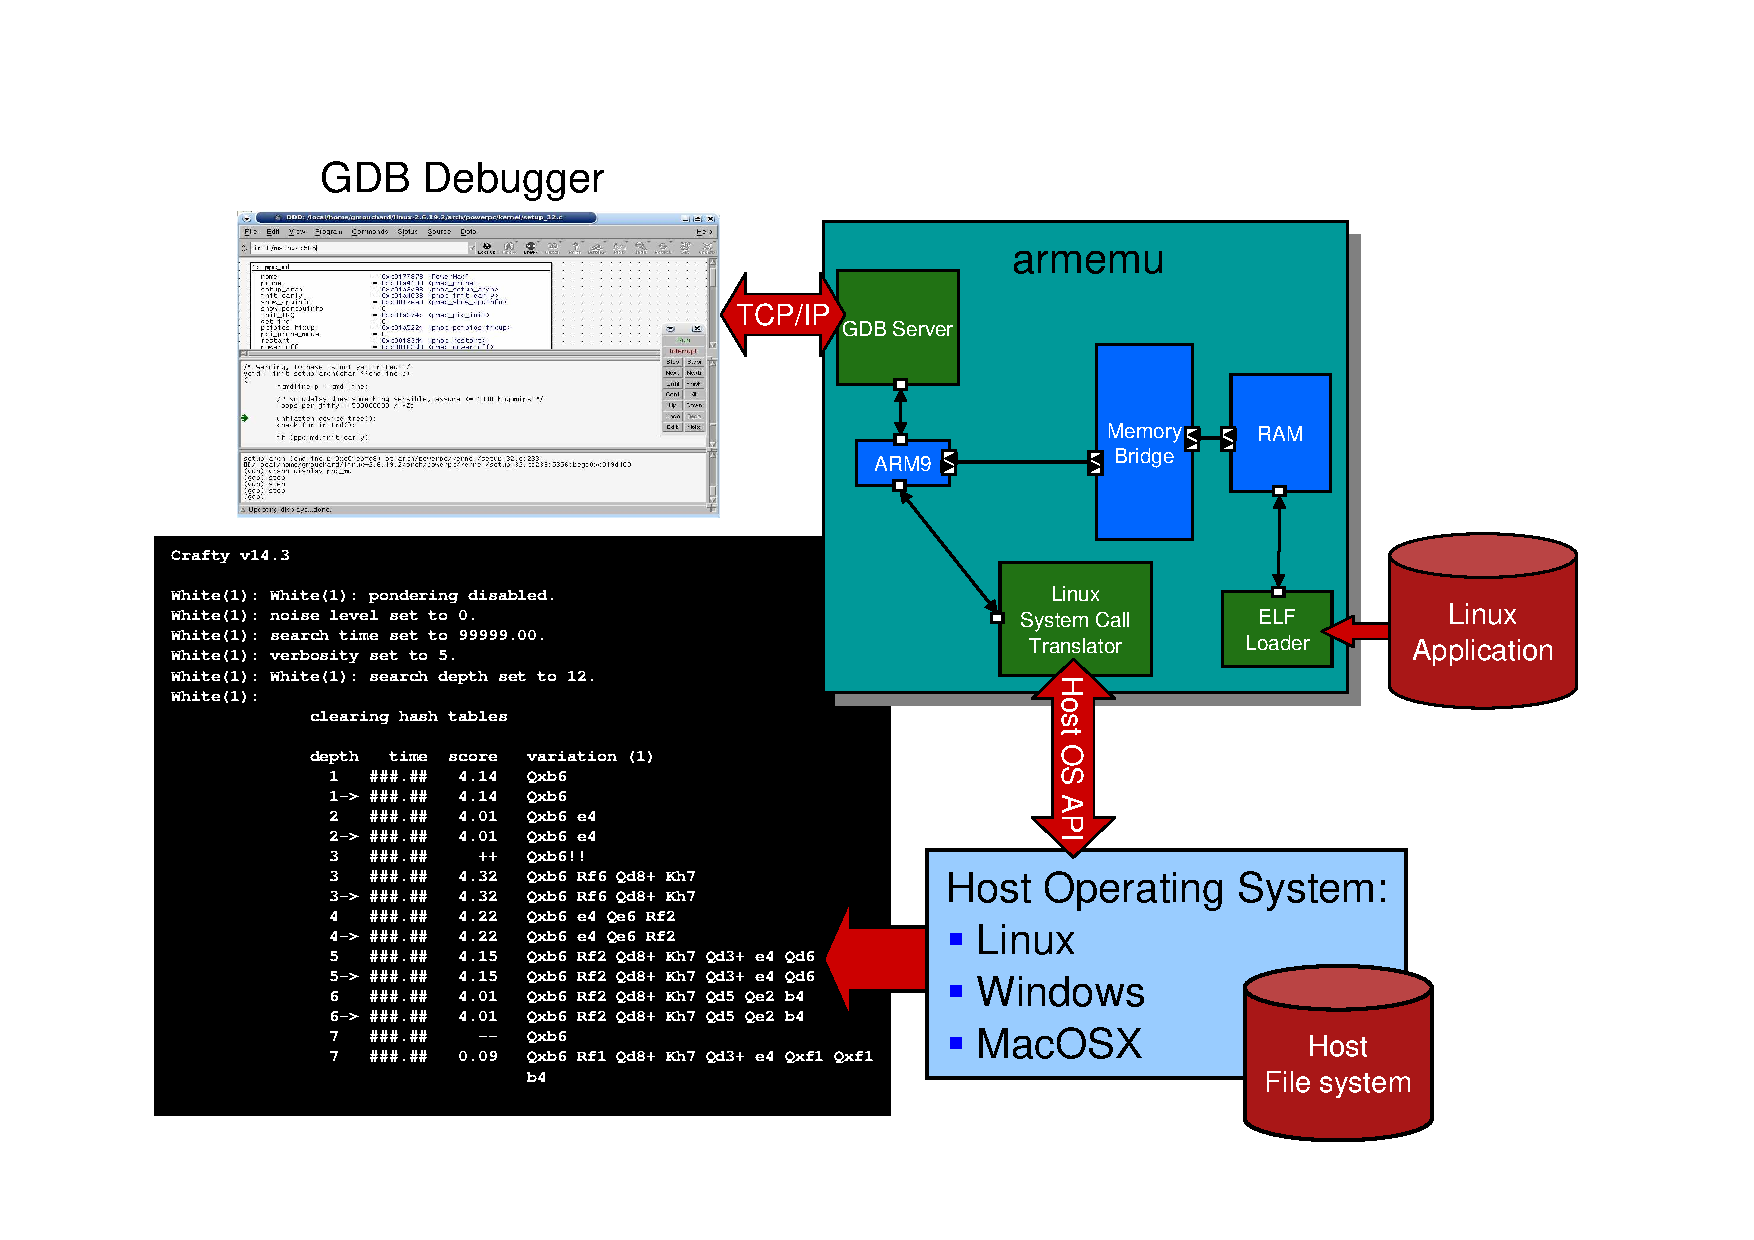
\includegraphics[width=\textwidth]{armemu/fig_armemu.pdf}
	\end{center}
	\caption{armemu simplified schematic.}
	\label{fig:armemu_system}
\end{figure}

Four different versions of the armemu simulator are provided:
\begin{itemize}\addtolength{\itemsep}{-0.40\baselineskip}
\item armemu: the main version. This version of the simulator includes caches, which increases the processor and simulator performance.
\item armemu-nocache: a version of the simulator without caches. Simulation (and processor) speed is greatly reduced because all the memory accesses must go to the memory system, they are not cached.
\item armemu-debug: identical to armemu, but provides lots of debugging information. Useful when modifying the code of the simulator to have a indeep view of what is happening in the simulator.
\item armemu-nocache-debug: identical to armemu-nocache, but provides lots of debugging information.
\end{itemize}

\section{Simulated configuration}

The simulator is composed of the following modules:
\begin{itemize}\addtolength{\itemsep}{-0.40\baselineskip}
\item ARM CPU configured as an ARM9
\item Simple bus to memory bridge
\item memory
\end{itemize}

The simulator uses the following services:
\begin{itemize}\addtolength{\itemsep}{-0.40\baselineskip}
\item ELF loader
\item GDB Server
\item Inline debugger
\item SystemC Time
\item Host Time
\end{itemize}

\section{Using the simulator}

Usage: \texttt{armemu [<options>] <program> [program arguments]}

     'program' is statically linked ELF32 ARM Linux program

Options:
\begin{itemize}
\item Starting the inline debugger
\texttt{--inline-debugger}
\texttt{-d}

\item Starting a GDB server
\texttt{--gdb-server <TCP port>}
\texttt{-g <TCP port>}

The GDB server will wait for a GDB client connection on the specified TCP port.

\item Using <arch file> as architecture description file for GDB server
\texttt{--gdb-server-arch-file <arch file>}
\texttt{-a  <arch file>}

\item Defining the number of instructions to simulate before exiting
\texttt{-i <count>}
\texttt{--max:inst <count>}

\item Enabling compression (gzip format) of the logger output

\texttt{-z}
\texttt{--logger:zip}

\item Redirecting the logger output to the standard error output

\texttt{-e}
\texttt{--logger:error}

\item Redirecting the logger output to the standard output

\texttt{-o}
\texttt{--logger:out}

\item Creating message spies (requires one log to work)
\texttt{-m}
\texttt{--logger:message\_spy}

\item Redirecting the logger output into a file

\texttt{-l <file>}
\texttt{--logger:file <file>}

\item Displaying the integrated help

\texttt{--help}
\texttt{-h}

\end{itemize}